\section{Motivation \& Background}

\begin{frame}{Model-based summaries of health vs disease}
	\centering
	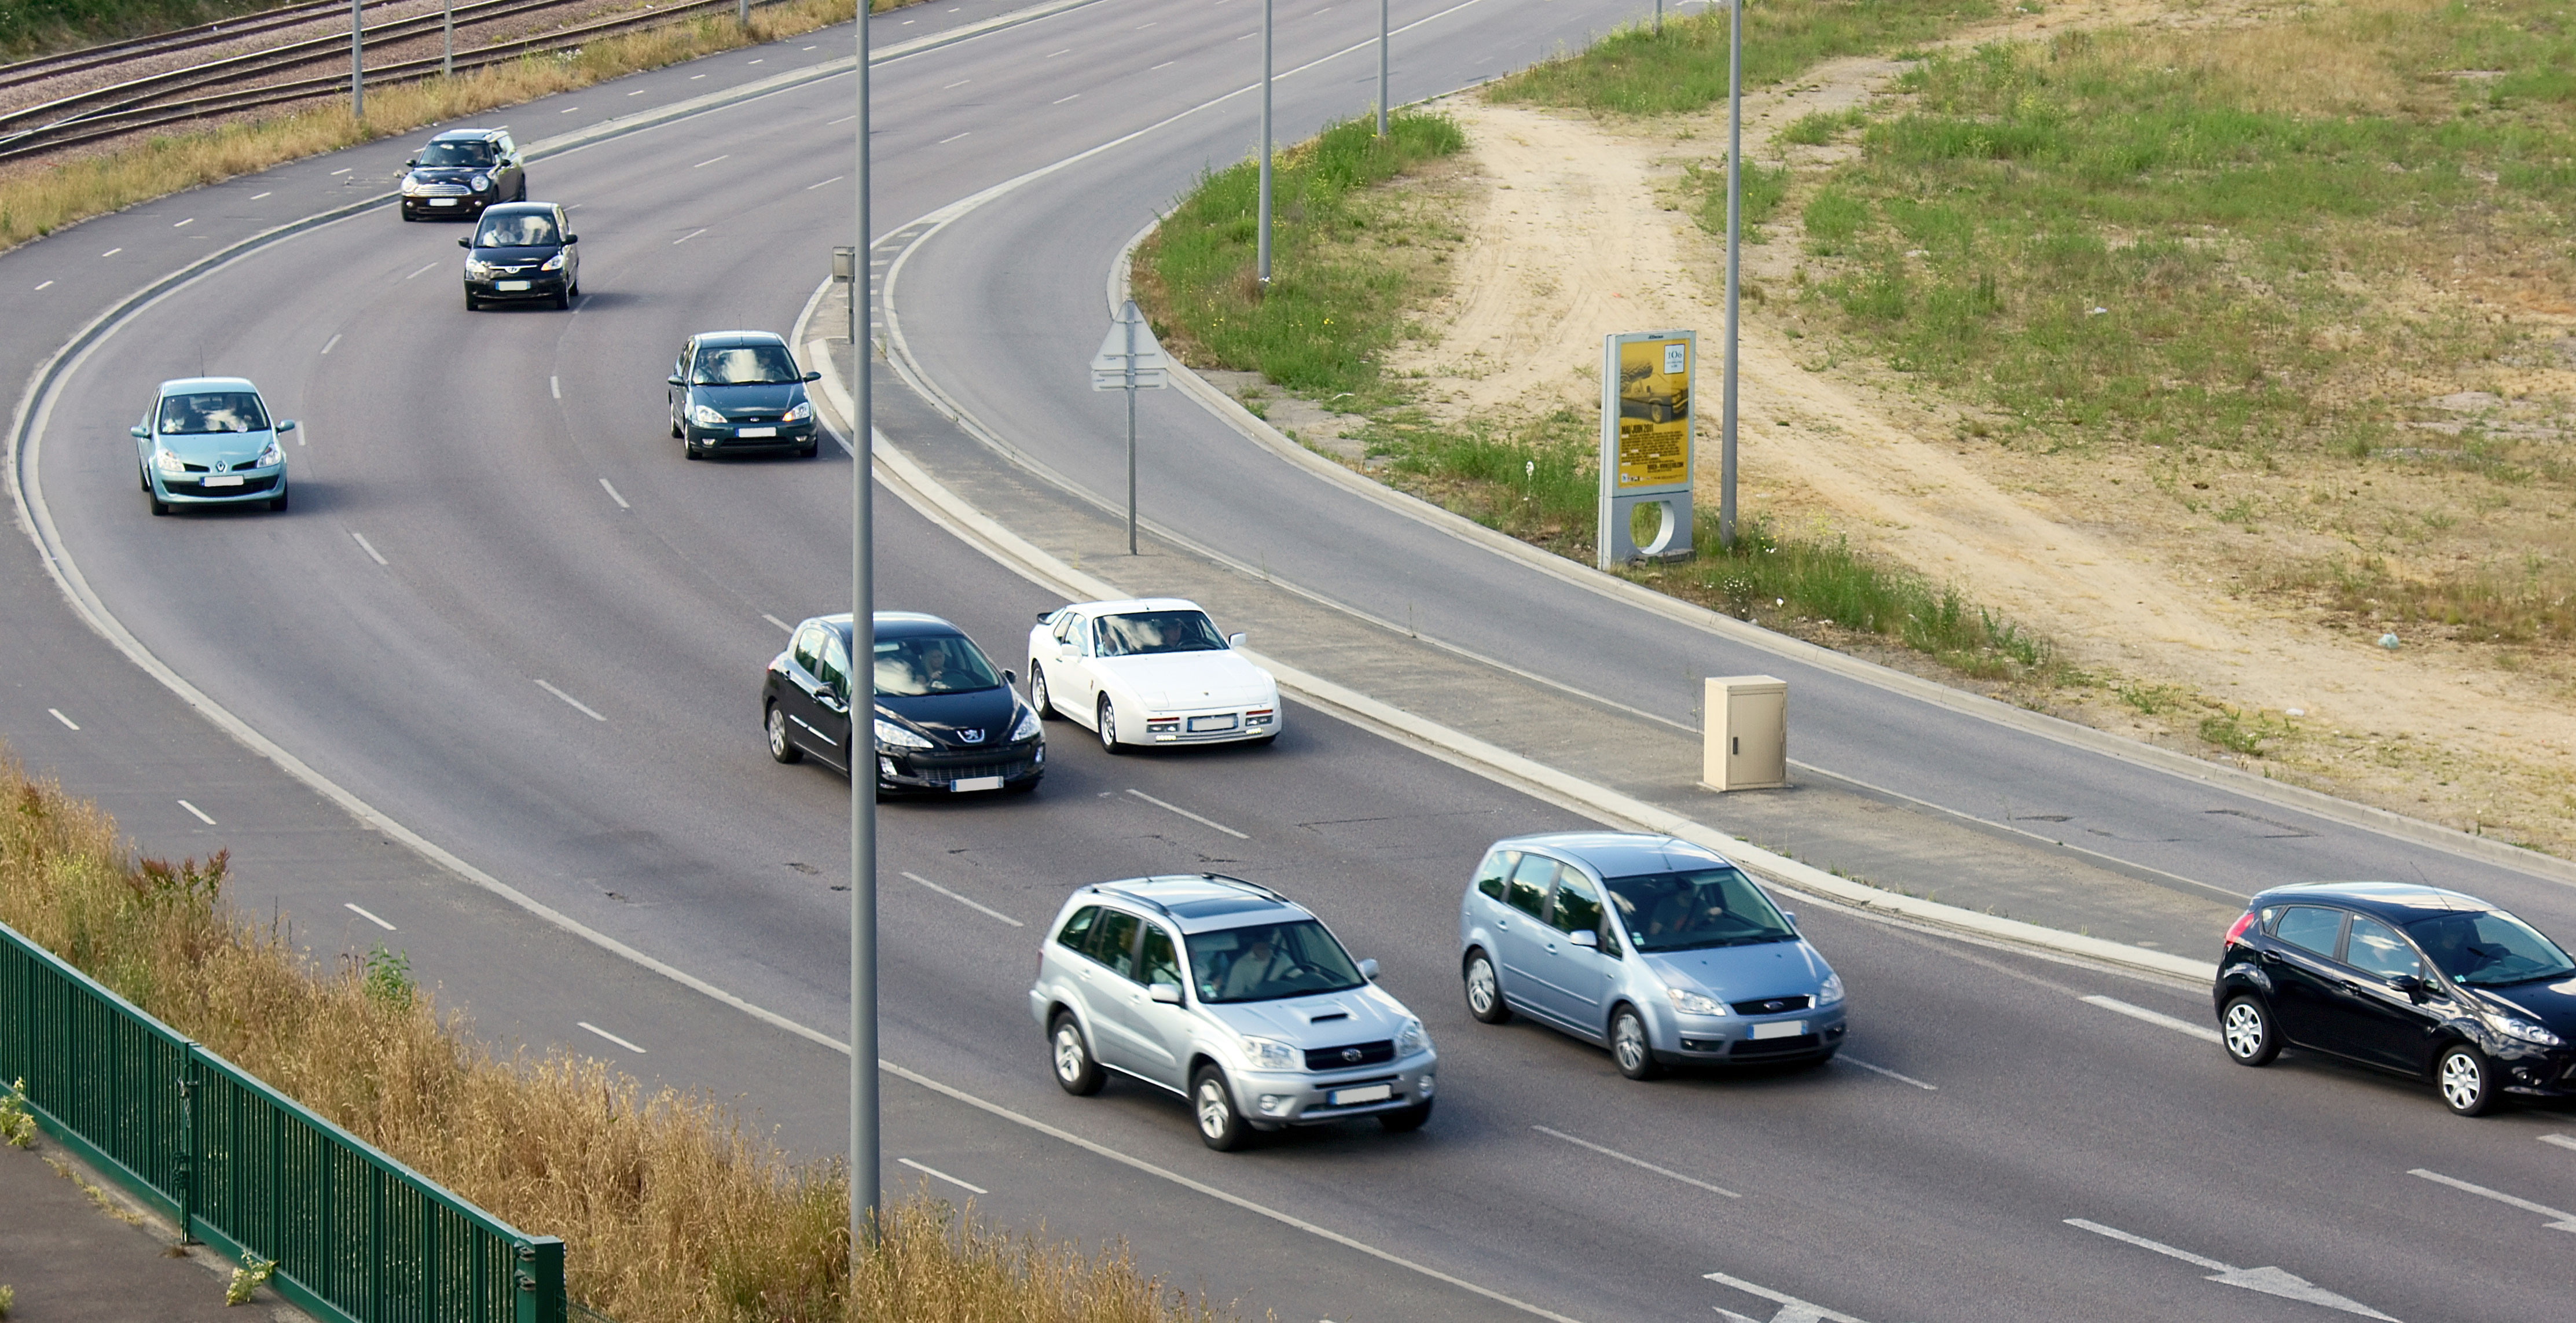
\includegraphics[width=0.5\textwidth]{media/cars_driving}\nakedfootnote{flickr:zigazou76 CC BY 2.0}
	% \includegraphics<1>[height=0.5\textheight]{media/garfield_without.png}\nakedfootnote{flickr:zigazou76 CC BY 2.0}
	% \uncover<2>{
\includegraphics[height=0.5\textheight]{media/garfield.png}\nakedfootnote{flickr:zigazou76 CC BY 2.0}}
	\note<1>{
		Let's draw an analogy for healthy vs diseased dynamics: safe vs dangerous driver.
		\begin{enumerate}
			\item static vs temporal: in defensive driving, want to keep staggered position. In static view, minivan driver is dangerous but in temporal view may be healthy as is simply passing the suburu.
			\item unit vs population: consider the black sedan following the minivan. If it maintains a consistent following distance by accelerating and braking, then a safe driver, but in a vaccuum with no information of other cars, looks completely erratic.
		\end{enumerate}
	}
	\uncover<2>{
		\makebox[\textwidth][c]{%
			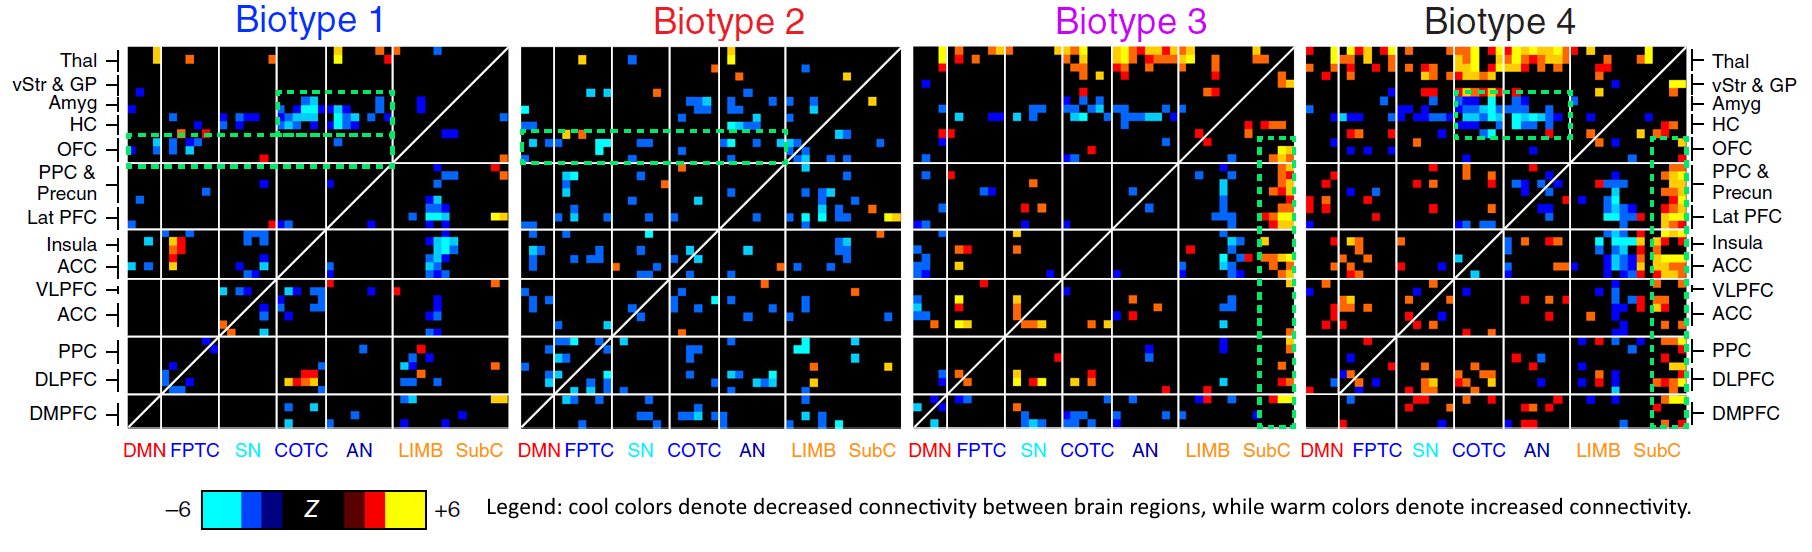
\includegraphics[width=1.1\textwidth]{media/depression_heatmap}
		}\nakedfootnote<2>{Drysdale, Grosenick, et al. \emph{Nature Medicine}. 2016}
	}
	\note<2>{
		Four functional connectivity "biotypes" from fMRI study of depressed patients. Has no notion of time (one true underlying phenotype capturing different snapshots?), and is not a causal model--where should we stim to nudge dynamics back towards health?

		Applications:
		\begin{itemize}
				\item muck with gene, a lot changes $\rightarrow$ create summary
				\item ``outlierness" of brain dynamics
				\item model gives reduction of whole data
		\end{itemize}

		Bern \& Molley  2013 for reliability of resting state fMRI.

		\textbf{transition:} lack of spatial resolution motivates jump model organism where we can observe whole-brain at cellular resolution.
	}
\end{frame}{}

% \begin{frame}{Goal: causal inference of neuronal computation}
%     \begin{center}
%         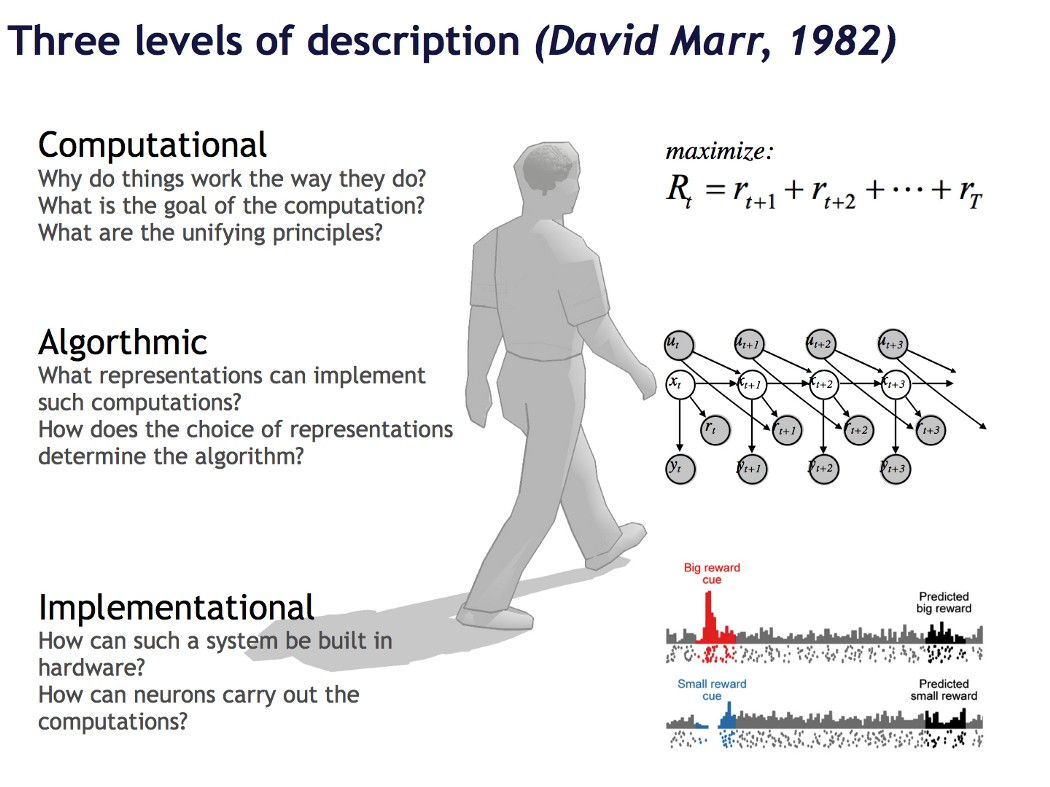
\includegraphics[height=0.9\textheight]{media/marr_levels.jpg}
%         \footnote{Rebbeca Wicker. \emph{Noam Chomsky, Linguistics and AI}. 2017}
%     \end{center}{}
% 		\note{Finding the goal of the computation is not always possible--e.g. resting state. So we use a surrogate goal: prediction of future brain activity. With this, we can create descriptions at the algorithmic and implementational levels.}
% \end{frame}{}

\begin{frame}{Challenge: high underlying complexity}{as shown by partial zebrafish projectome}
				\centering
				\begin{figure}
					\adjincludegraphics[trim={0 {.39\height} 0 0},width=0.55\textwidth,clip]{media/projectome.jpg}
					\caption{$\sim80,000$ neurons at 7 days post fertilization (dpf)\nakedfootnote{Hildebrand, Cicconet, et al. \emph{Nature} 2017}\nakedfootnote{Hill, Howard, et al. 2003}}
				\end{figure}

    % \begin{multicols}{2}
    %     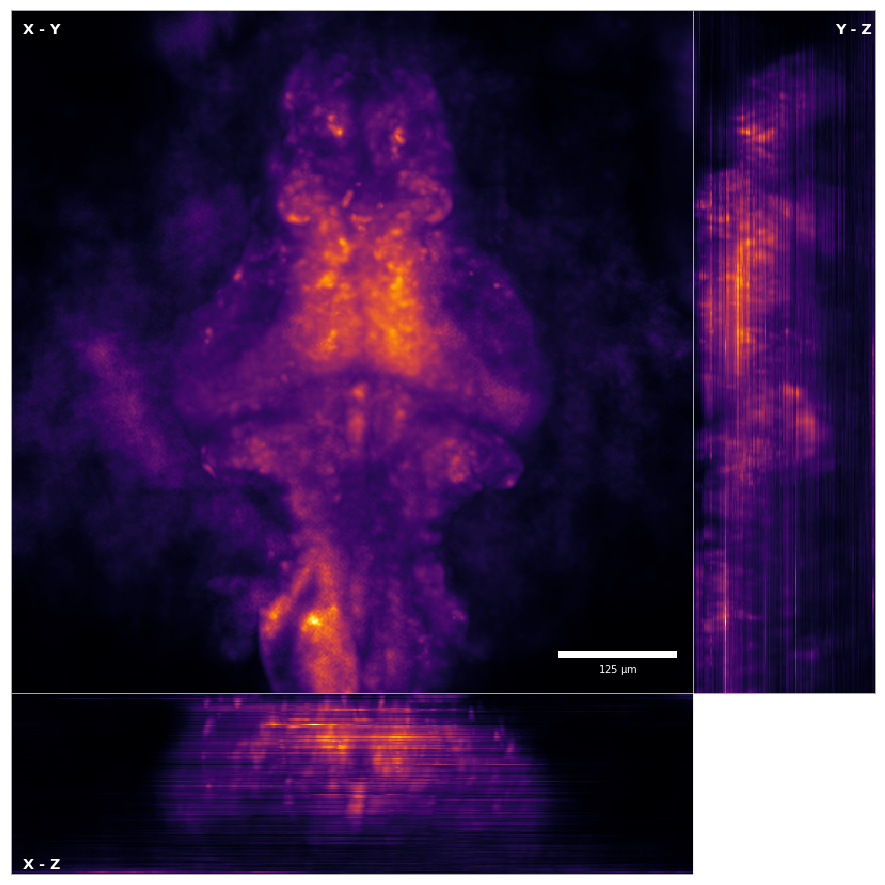
\includegraphics[width=0.49\textwidth]{media/lfm.png}
    %     \,
    %     1.4 TB/hr.\nakedfootnote{Noah Young. \emph{unpublished}. 2019}
		% 		\uncover<2>{
	  %       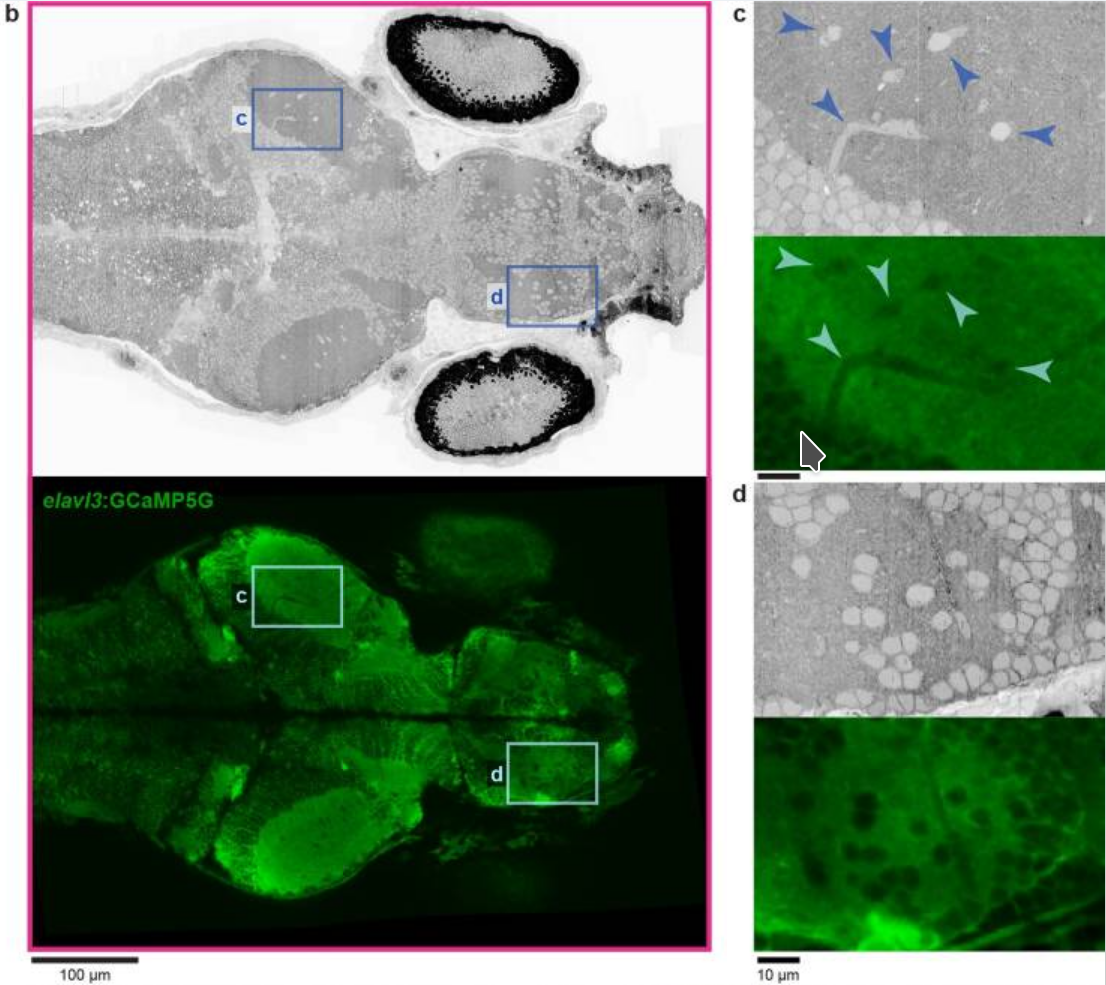
\includegraphics[width=0.5\textwidth]{media/em.png}
	  %       \,
	  %       20-100 TB / mm\textsuperscript{3}.
		% 		}
    % \end{multicols}
		% \nakedfootnote<2>{Hildebrand et al. \emph{Nature}. 2017}
\end{frame}{}

\begin{frame}{Opportunity: massive datasets}{Whole-brain imaging \& stimulation}
				\centering
		    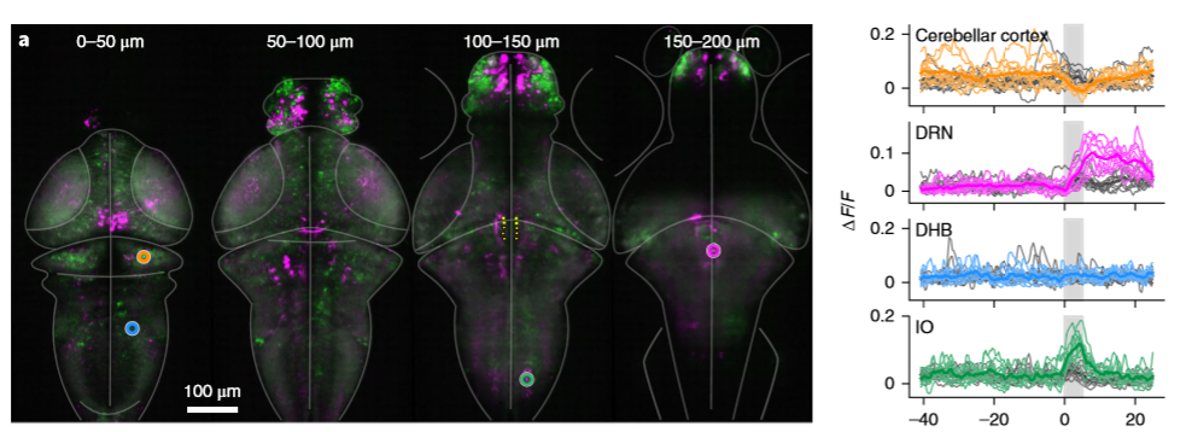
\includegraphics[width=1.1\textwidth,center]{media/drn_opto}
        \linebreak
        \textbf{left:} increase in activity (green), decrease in activity (magenta), optogenetic stimulation sites (yellow)
				\textbf{right:} dorsal raphe nucleus (DRN), dorsal hindbrain (DHB), and inferior olive (IO)
				\nakedfootnote{Vladimirov, Wang, et al. 2018}
\end{frame}


\begin{frame}{Validate modeling results through comparison to well-characterized Mauthner circuit}
	\centering
	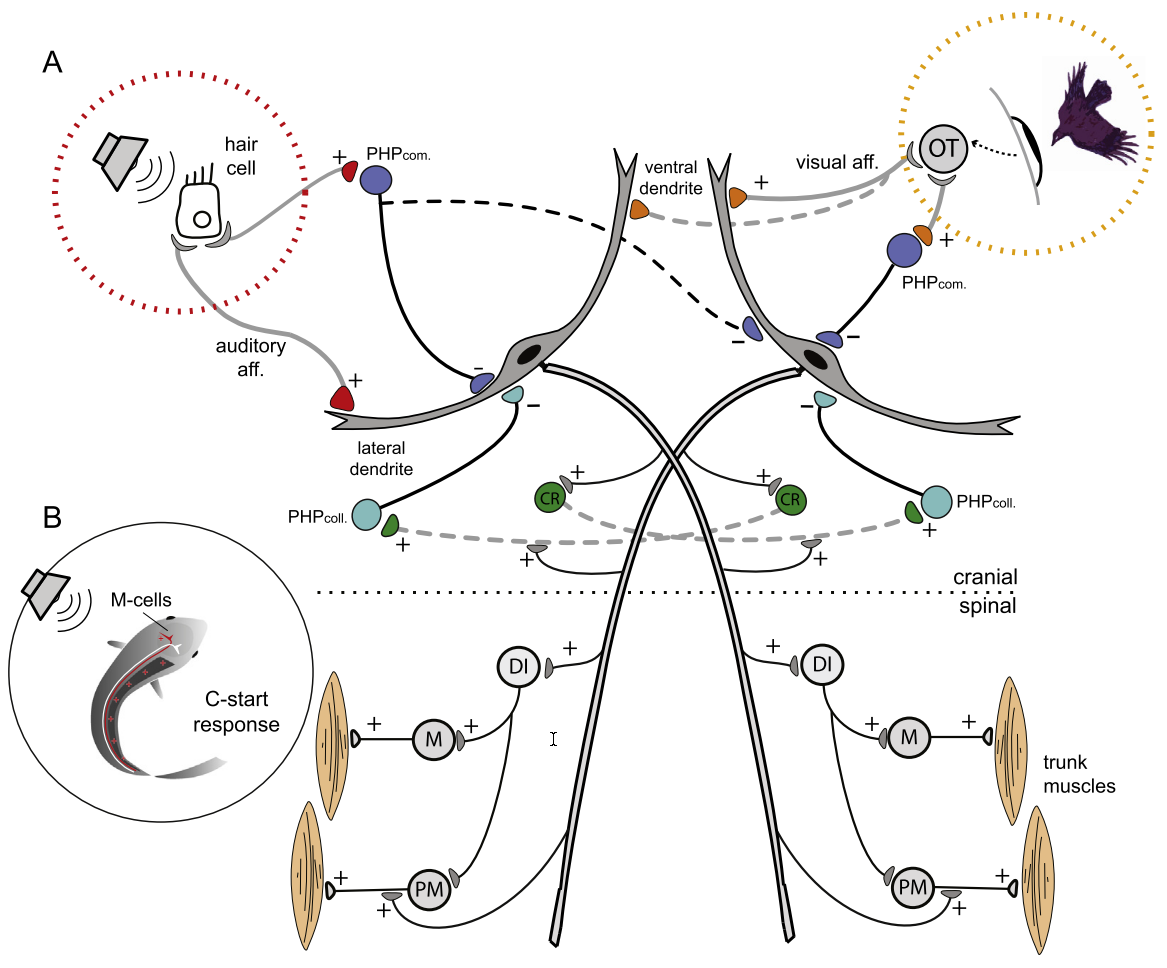
\includegraphics[height=0.9\textheight]{media/mauthner_circuit.png}
	\nakedfootnote{Medan \& Preuss, 2014}
	\note{M-cell AP $\rightarrow$ negative field potential of 20–40 mV close to axon hillock \tiny Schematic shows the paired Mauthner cells (M-cells), their visual and statoacoustic inputs and cranial inhibitory networks. Each M-cell receives bilateral visual inputs and ipsilateral auditory inputs. The schematic shows only the left auditory afferents (red) and the right visual afferents (orange). The auditory pathway is direct, as hair cells activate auditory nerve afferents with synapses on the M-cell’s lateral dendrite and also excite bilaterally-projecting feedforward inhibitory interneurons, the commissural PHP cells (blue). The collateral PHP neuron population (coll., light blue) mediates recurrent (feedback) inhibition triggered by firing of either ipsilateral or contralateral M-cells that is conveyed through the cranial relay neurons (CR, green). The polysynaptic visual pathway conveys information from the retina to the optic tectum (OT) which sends afferents that contact both M-cells ventral dendrite. M-cell axons exit the medulla through the spinal cord to make direct contact with primary motoneurons (PM) and indirect contanct with other motoneurons (M) through a set of interneurons (DI). Spinal inhibitory networks and cranial motoneurons are omitted to simplify the schematic. A single action potential in one of the M-cell produces contraction of contralateral trunk muscles producing the characteristic C-shape that initiates the startle response or C-start (B).}
\end{frame}

%
% \begin{frame}{Artificial intelligence}{motifs through space and time}
% 		\centering
% 		\makebox[\textwidth][c]{%
% 			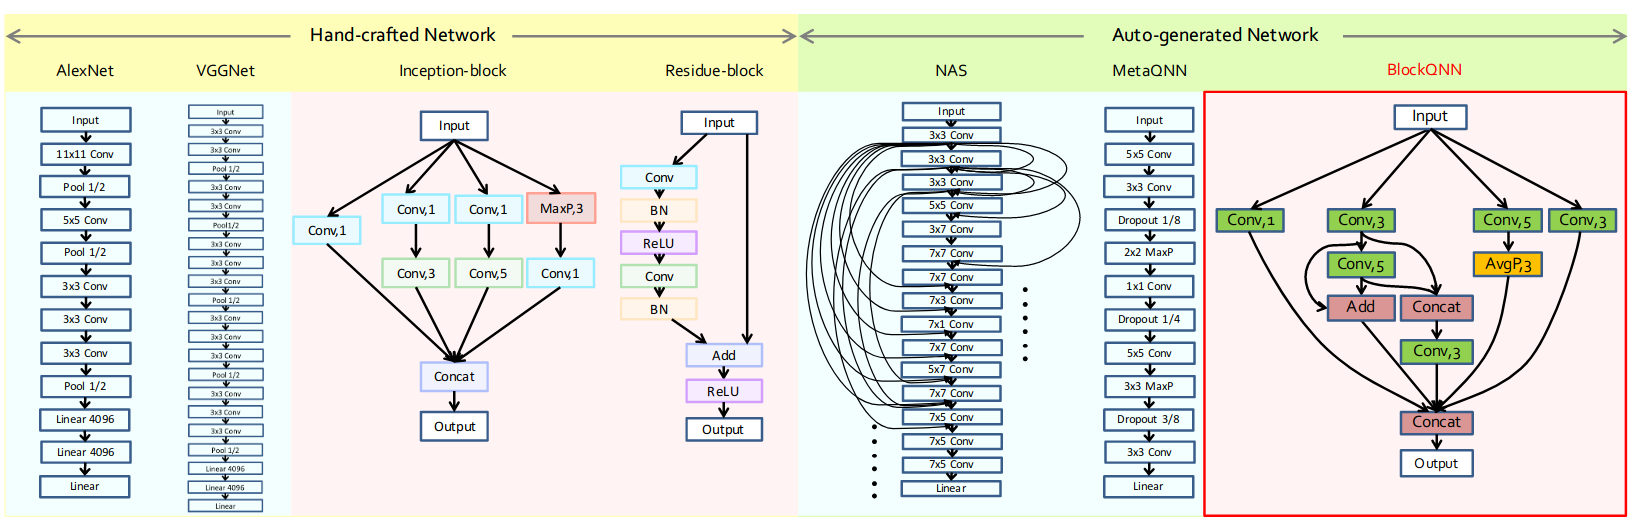
\includegraphics[width=1.1\textwidth]{media/block_search}
% 		}\nakedfootnote{Zhong, et al. \emph{CVPR`18}}
% 		\note[item]{We may discover neuroscience motifs that are useful for AI.}
% 		\note[item]{Fitting neural data as a regularizer}
% \end{frame}{}
